\documentclass[dvipdfmx]{jsarticle}
\usepackage{graphicx}
\usepackage{amsmath}
\title{公衆無線LANを用いたHTTPS通信に対する\\MITM攻撃の新手法の開発とその実装}
\author{神戸大学工学部電気電子工学科 木村圭一朗}
\begin{document}
    \maketitle
    \begin{abstract}
        \ 昨今のネットワークの著しい普及により,屋外で利用できるネットワークの需要が拡大している.\
        その需要に応える通信インフラとして公衆無線LANがあり,公共のあらゆる場でその整備が進んでいる.\
        しかし,セキュリティ面での懸念は以前として残っている.\
        利用した公衆無線LANが通信の傍受を目的とした悪性のものである可能性は,その懸念の一例である.
        屋外で手軽にインターネットを利用できる反面,ユーザーたちはその公衆無線LANの提供元を確認することはほとんどないだろう.\
        近年は通信内容が暗号化されたHTTPS通信が主流になり,中間者攻撃も簡単に実行できないが,公衆無線LANを利用した通信の場合はそれが可能になる場合がある.\
        本稿では,主にその手法と具体的な検証結果について記す.
        \newline
    \end{abstract}
    \tableofcontents
    \clearpage
    \section{序論}

    \section{前提知識・用語}
        本稿を進めるにあたり,必要であると思われる前提知識及び用語を以下に記す.
        \subsection{通信関連について}
            \begin{description}
                \item[HTTP]\mbox{}\\
                    Hypertext Transfer Protocolの略であり,主にブラウザとサーバ間でWeb情報のやりとりを目的としたアプリケーション層プロトコルを指す.\
                \item[HTTPS]\mbox{}\\ 
                \item[中間者攻撃(man-in-the-middle attack)]\mbox{}\\ 
                    通信を行う二者の通信に対して,第三者がプロキシサーバーの様に中継を行う事で,通信内容の傍受・改竄を行う攻撃手法を指す.\
                    国内外を通じてインターネットの普及に伴う公衆無線LANの設置が進んでいるが,これらの中に悪意を持ったアクセスポイントがあれば,そこを起点として通信内容が盗み見られる可能性がある.
            \end{description}
        \subsection{無線LAN関連について}
            \begin{description}
                \item [SSID]\mbox{}\\
                    Service Set Identifierの略で,無線LANの識別子を指す.
                \item [Captive Portal]\mbox{}\\
                    無線及び有線ネットワークに接続したユーザーが,ネットワークへのアクセスを許可される前に表示される認証ページを指す.\
                    ユーザーは,アクセス許可に必要な情報の入力或いは利用規約への同意を行い,その認証を行ってもらう事でインターネットへのアクセスが可能になる.\
            \end{description}
        \subsection{その他}
            \begin{description}
                \item[HTML]\mbox{}\\
                \item[ハイパーリンク]\mbox{}\\  
            \end{description}
    \section{目標}
        本研究の目標を以下に示す.
        \begin{quote}
            偽のSSIDを用いた公衆無線LANからクライアントと正規サーバとの通信に割り込み,デバイスに警告を出さずに通信の傍受・改竄を行う事.\
        \end{quote}
        デバイスに警告を出さないという点について,ここではHTTPS通信を想定する.\
        通常,ユーザーが利用するブラウザでは,その通信先が正規のもの,つまり第三者が複製した偽物のサイトではないことを確認する為に,名前検証を行う.\
        名前検証とは,通信のドメインとSSL証明書に記載されているドメインが一致しているかの確認を行う事であるが,この時用いられるSSL証明書を第三者が複製・改竄することは非常に困難とされている.\
        TODO:この説明ここじゃない気がするので構成考える.
    \section{前提条件と仮説}
        \subsection{前提条件}
            今回,MITM攻撃を仕掛けるにあたり以下の前提条件を設ける.\\
            \\
            利用者は
            \begin{itemize}
                \item 偽SSIDを有する無線LANアクセスポイント(以下,AP)を使用する.
                \item HTTPS通信で任意のサイトを閲覧する.
                \item 通信先を確認しない.
            \end{itemize}
             まず,偽SSIDを有するAPを利用するという前提条件について説明する.\
            攻撃者が利用者の通信の内容を盗み見る為には,利用者を攻撃者が用意したAPへ接続させる必要がある.\
            しかし,通常の公衆のAPのSSIDは提供している施設や会社の名前に関連したものが多く,利用者も提供元の名前に関連したSSIDを有するAPに接続を試みる.\
            従って,攻撃者が用意したAPのSSIDも,利用者が施設や会社が提供したWiFiであると誤認させる様なSSIDを用いるという前提が必要である.\\
             次に,利用者はHTTPS通信でサイトを利用するという条件について,これは現在のWebサイト,特に個人情報などのセンシティブな情報を扱うようなWebサイトは常時HTTPS通信を用いている点にある.\
            特に,中間者攻撃への対抗策としてHSTP(HTTP Strict Transport Security)という,サーバーがブラウザに対してHTTPS通信を強制する様な仕組みも実装されているものもある.\
            従って,通信内容に対して暗号化が施されていないHTTP通信を前提としての検証は現実的出ない為,HTTPS通信を想定する必要がある.\\
             最後に,通信先を確認しないという前提についてであるが,これは一般的な利用者の想定を意味する.\
            通常,ネットワークについての知識が深い利用者や,セキュリティリテラシーの高い利用者は,閲覧しているサイトのドメインなどを確認して,正規サーバと通信しているかを確認する事があるが,一般的な利用者はそのような確認は行わない.\
            本研究は公衆無線LANを用いる一般的な利用者を想定している為,通信先の確認は想定しない.\\
        \subsection{仮説}
            上記の前提条件をもとに,次の仮説を立てる.
            \begin{quote}
                ユーザーが攻撃者が用意した偽のSSIDを有する公衆無線LANを用い,そのCaptive Portal画面で表示された偽の検索エンジンからネットを利用した場合,\
                ユーザーの通信がHTTPS通信でも,攻撃者がその通信の盗聴・改竄が可能になる.
            \end{quote}
    \section{検証内容}
        \subsection{検証対象}
            MITM攻撃が可能か否かの検証にあたり,昨今急激な普及が見られるインターネット通販サイトを対象とした.その中でも国内ECモールの売上ランキング上位2つを占める「楽天」と「Amazon」を対象とした.\
            また,これ以降は,攻撃者が用意した悪意あるAPを「悪性AP」,通信の仲介に用いる攻撃者サーバを「悪性サーバ」をして説明する.
        \subsection{検証フロー}
            主な検証フローは次の通り.各フェースの具体的な説明は次のサブセクションに記述している.
            \begin{enumerate}
                \item CaptivePortalを検知させて,予め攻撃者が用意しておいたCaptive Portalサイトに誘導させる.
                \item Captive Portalサイトで表示された偽の検索エンジンから,被害者が検索したワードを悪性サーバで取得する.
                \item 攻撃者は取得したワードをバックエンドで検索し,その検索結果を取得.
                \item 取得したHTMLファイル内にあるハイパーリンクを書き換え,そのコピーを被害者に提示する.
                \item 以後,クリックしたURLを悪性サーバで取得する.
                \item 攻撃者は取得したURLを利用して正規サーバにアクセスする.
                \item 正規サーバから返却されたHTMLファイル内のハイパーリンクを書き換えたものを被害者に提示する.
            \end{enumerate}
        \subsection{実装}
            悪性サーバの実装はGolangで実装した.\
            以下に該当のGitHubリポジトリのリンクを載せている.\
            ここでは,検証フローの内容について具体的な実装内容を示す.\
            \subsubsection{1,2について}
                前提知識・用語のセクションでも記述したが,Captive Portalとは,インターネットを利用する際にそのユーザーの認証や利用規約に同意させる為に,一時的に外部との通信を制限して認証画面に飛ばす仕組み,或いはその認証ページを指す.\
                例えばカフェや飛行機,新幹線で提供されている公衆無線LANを利用した際などは,認証ページに飛ばされるという経験は決して珍しいものではない.\
                また,要求された認証が終えると,インターネットへのアクセスが許可され,予め用意された別のサイトに飛ばされる事もある.\
                今回はこの仕組みを利用する.\
                \begin{figure}
                    \centering
                    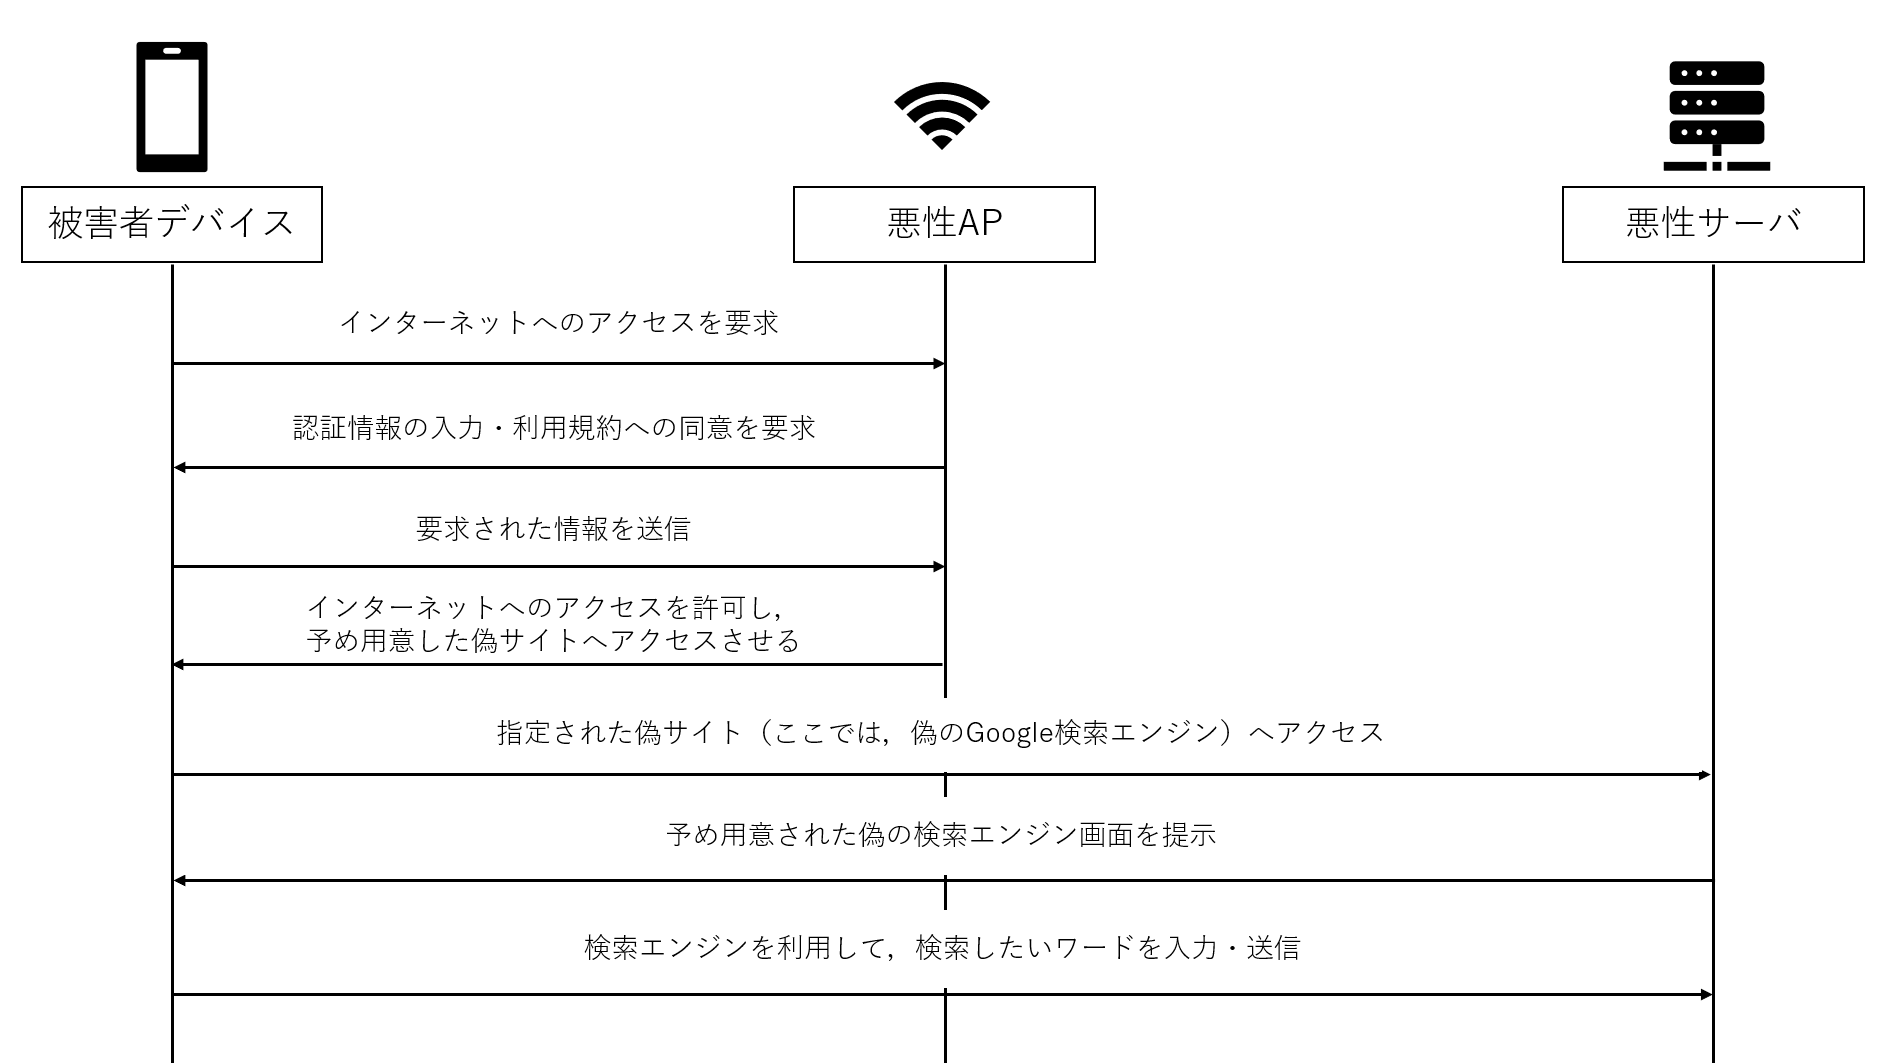
\includegraphics[width=15cm]{img/vc-vf-1-2.png}
                    \caption{偽のAPとCaptive Portalの仕組みを仕様して,偽の検索エンジンに飛ばすまでの挙動}
                    \label{flow-no12}
                \end{figure}
            \subsubsection{3について}
                ここでは,最も利用されている検索エンジンGoogleを用いた.\
                Googleでの検索結果を取得する為には,検索クエリを作成する必要がある.\
                基本的に任意のクエリ(query)に対して https://google.com/search?q=queryというURLがGoogleの検索URLとなっているが,クエリに空文字列が存在する場合は,その空文字列を+に置換する必要があることに留意しなければならない.\
                例えば,「神戸大学 工学部」と検索する場合には,そのURLはhttps://google.com/search?q=神戸大学+工学部となる.\
                このURLを叩くことで,正規サーバからの応答を取得・自動生成を行う(\ref{flow-no3}).\\
                \begin{figure}[pt]
                    \centering
                    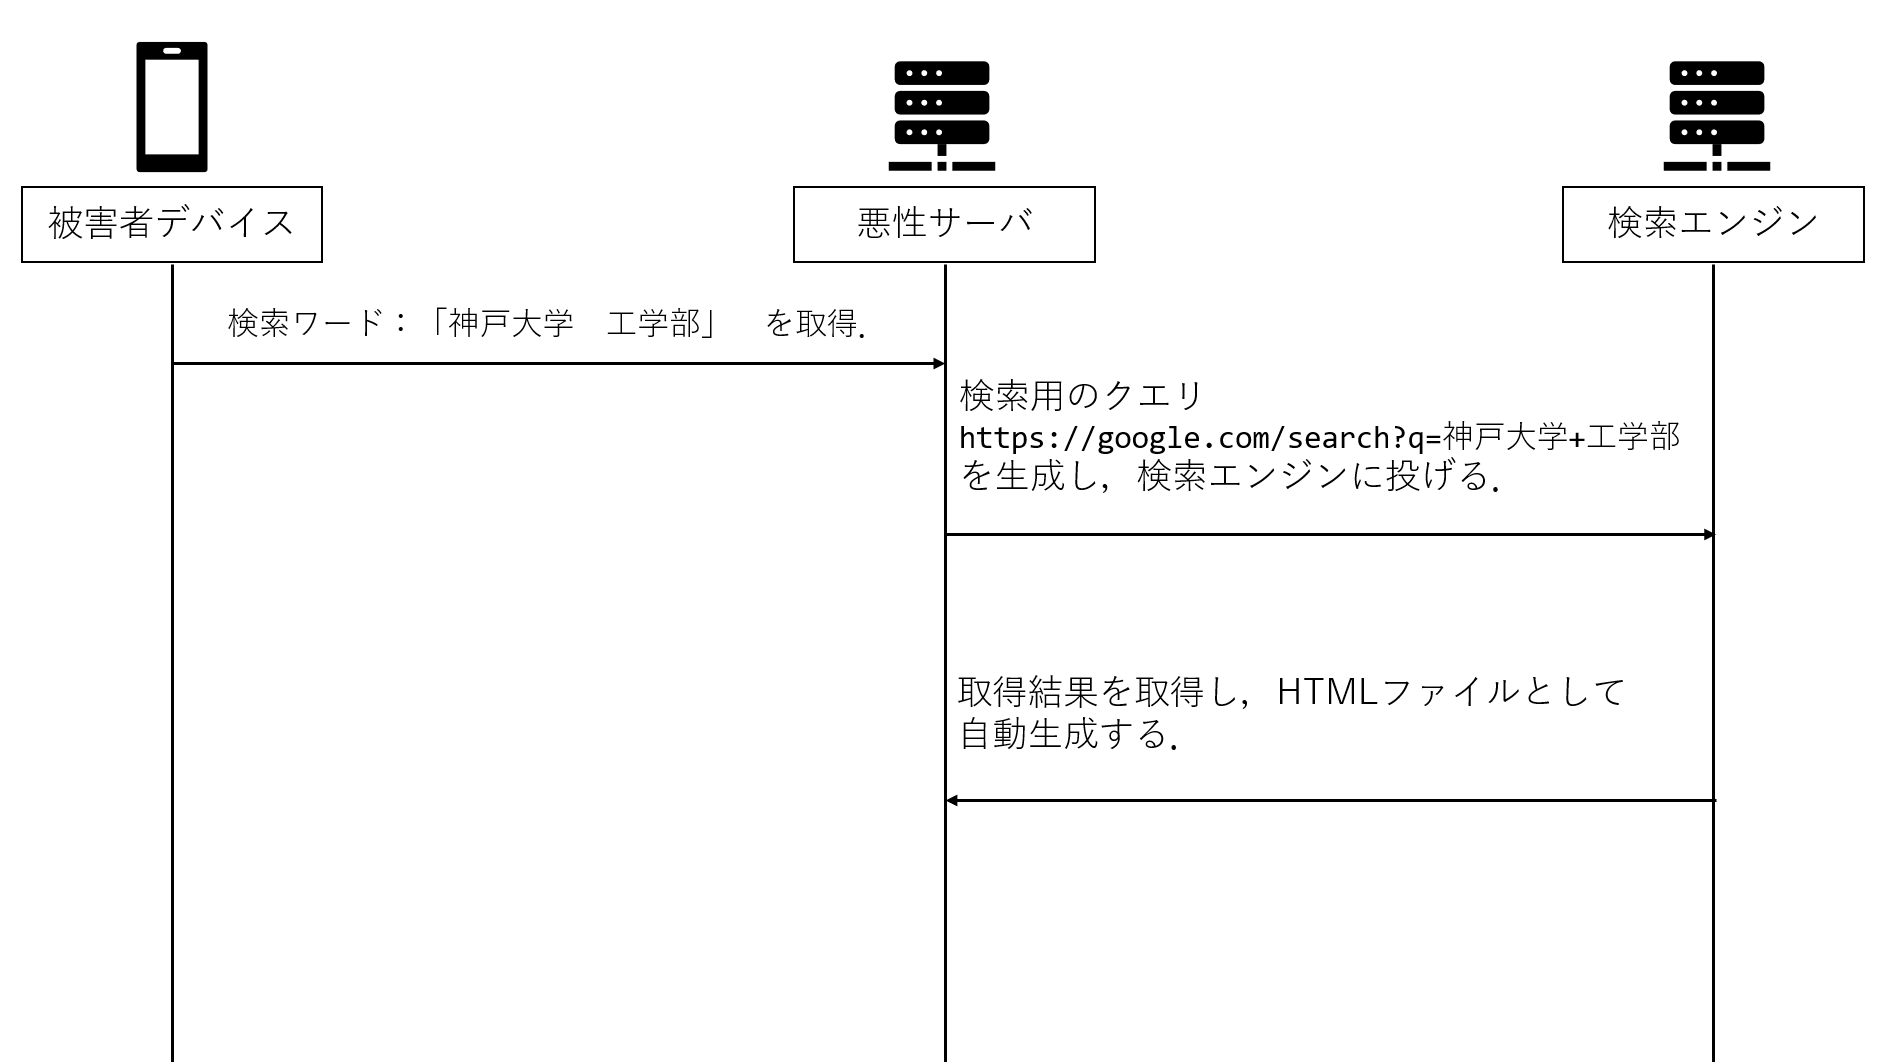
\includegraphics[width=15cm]{img/vc-vf-3.png}
                    \caption{検索ワードを取得してから,検索結果を取得するまでの流れ}
                    \label{flow-no3} 
                \end{figure}
                \clearpage
            \subsubsection{4,5について}
                取得したHTMLファイル内にあるハイパーリンクがそのままであれば,悪性サーバではなく正規サーバとの通信に切り替わってしまう.\
                従って,既存のURLを悪性サーバへ通信するように書き換え,且つ既存のURLを正確に抽出する必要がある.\
                これを実現する為には,既存のハイパーリンクをルールに則って書き換える必要がある.\
                具体的に,https://example.comというURLに対して処理を行うことを考える.\
                サーバには予め,URLを受け取る為のエンドポイントを設置する.今回の場合は「/templates」というエンドポイントに対して,「url」というパラメータを受け取るものとする.\
                このエンドポイントに対して適切にURLを飛ばすために,サーバ側で予め/templates?url=https://example.comのように書き換える.\
                その結果,被害者に提示したHTMLファイル内にあるハイパーリンクをクリックすると悪性サーバに飛び,且つサーバ側で遷移しようとしたページのリンクを取得できる.
                \begin{figure}
                    \centering
                    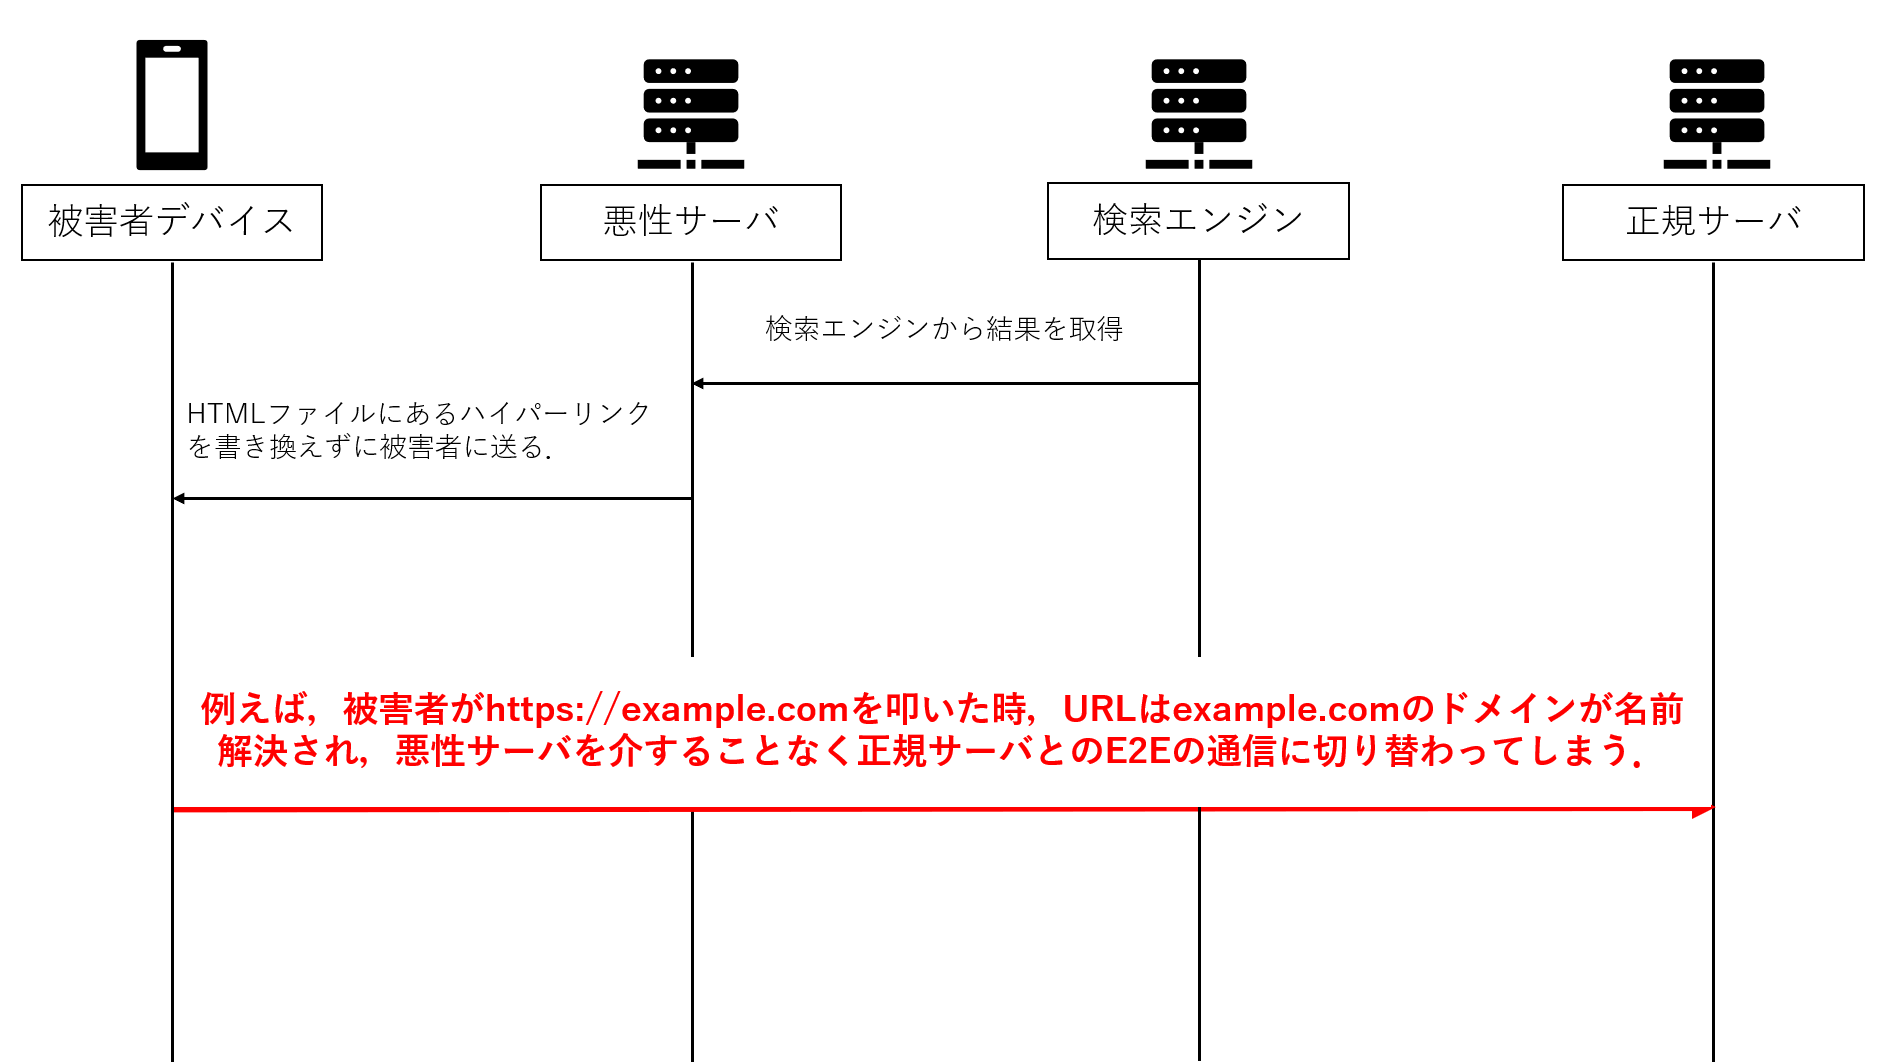
\includegraphics[width=15cm]{img/vc-vf-4-5-00.png}
                    \caption{HTMLファイル内のハイパーリンクを書き換えなかった場合の挙動}
                    \label{flow-no45-00}
                    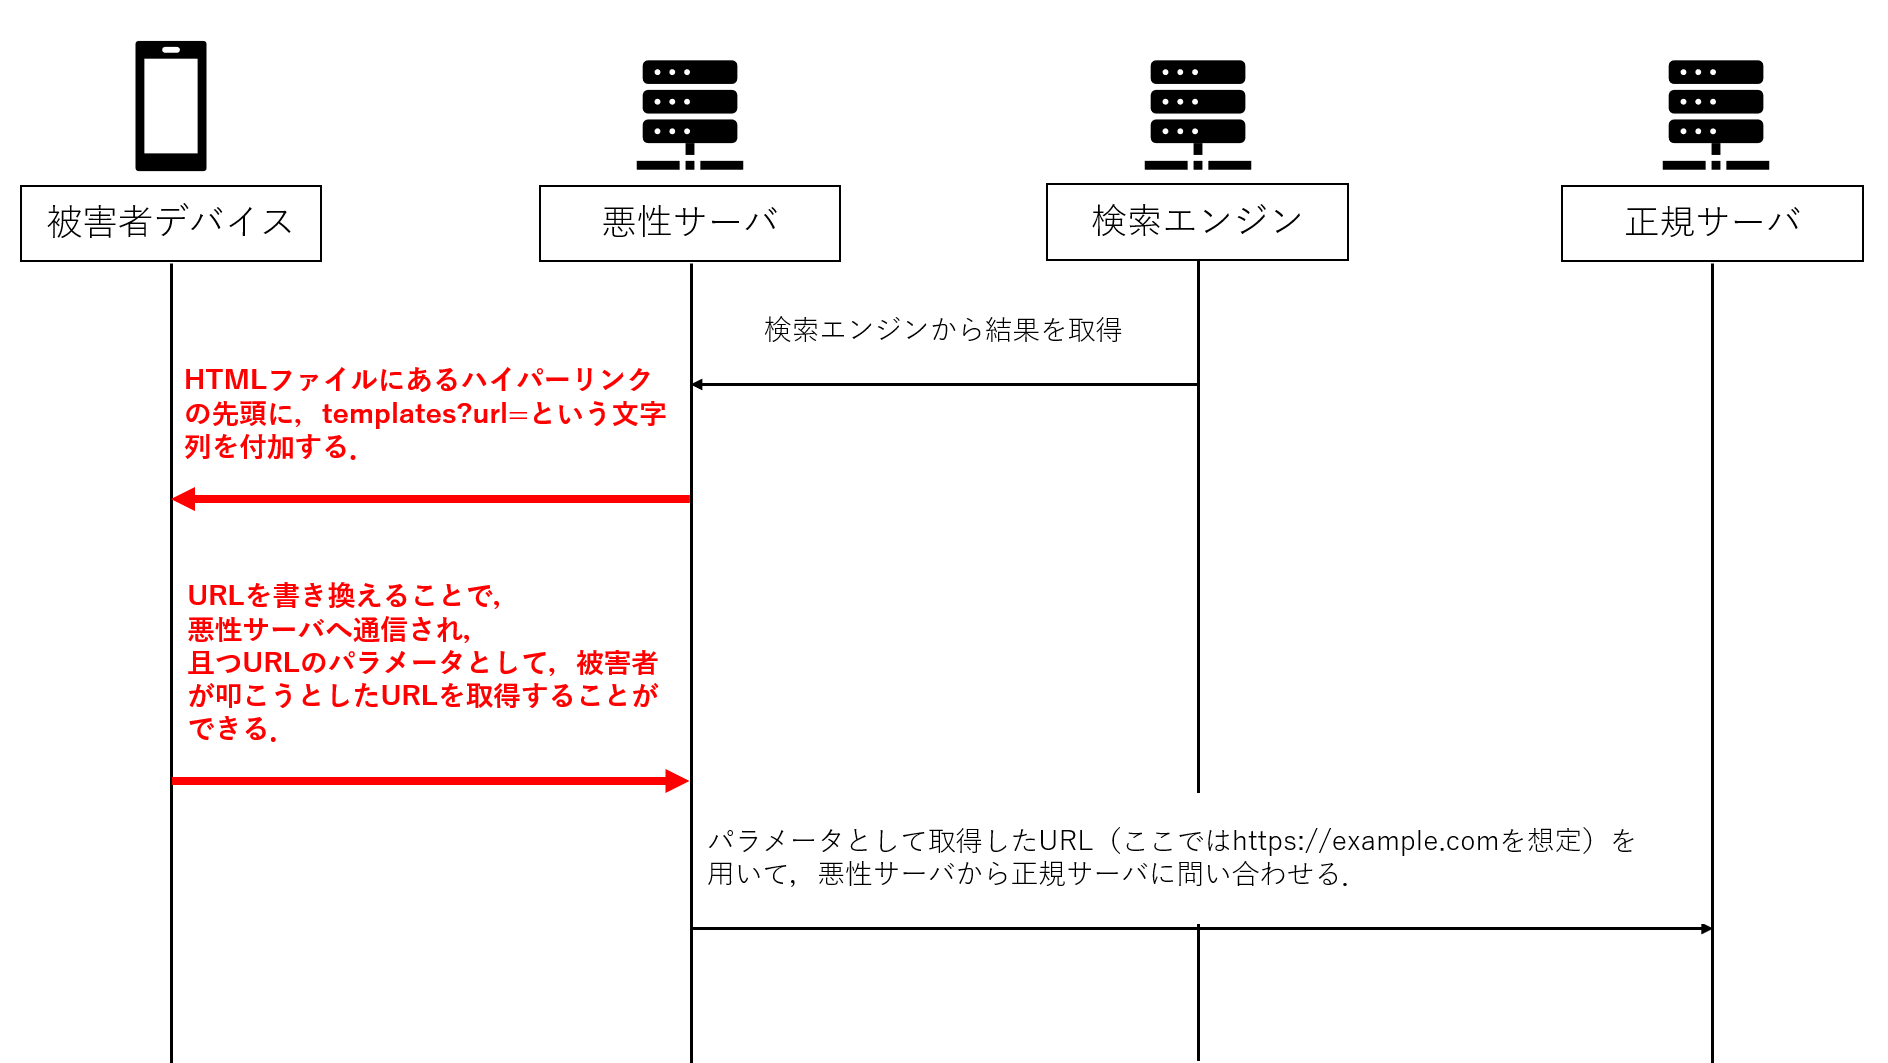
\includegraphics[width=15cm]{img/vc-vf-4-5-01.png}
                    \caption{HTMLファイル内のハイパーリンクを書き換えた場合の挙動}
                    \label{flow-no45-01}
                \end{figure}
            \subsubsection{6,7について}
                フローの4と5で得た正規URLを用いて,バックエンドで正規サーバとの通信及びHTMLファイルの取得を行う.\
                通常の通信であればHTMLファイルの取得のみでよいが,個人アカウントへのログインを行う際は,そのIDとパスワードを取得し且つ得られた情報と実際に登録されている情報との整合性の確認を行わなければならない.\
                登録情報の整合性に関しては,取得した個人情報を攻撃者が手動で入力・確認を行わず,バックエンドでブラウザのインスタンスを生成して入力・確認を行う.\
                この処理に関して,ChromedpというGolangで実装されているパッケージを用いた.\
                具体的な実装についてはGitHubレポジトリを参照して頂きたい.ここでは,処理の流れを以下に簡単に示す.
                \begin{enumerate}
                    \item Chromeインスタンスを生成する.
                    \item 指定URLを叩き,JS Pathを指定して該当部分に取得したIDやパスワードを入力する.
                    \item 個人情報の入力が完了すれば,同じくログインボタンのJS Pathを指定してログイン処理を行う.
                    \item 正規サーバに情報を整合させ,返却されたHTMLファイル内のハイパーリンクを,4と5と同じ要領で書き換えて被害者に返却する.
                \end{enumerate}
                JS Pathの指定に関しては,予め正規サイトのログイン画面を見てから確認・指定をする必要がある.
                \begin{figure}
                    \centering
                    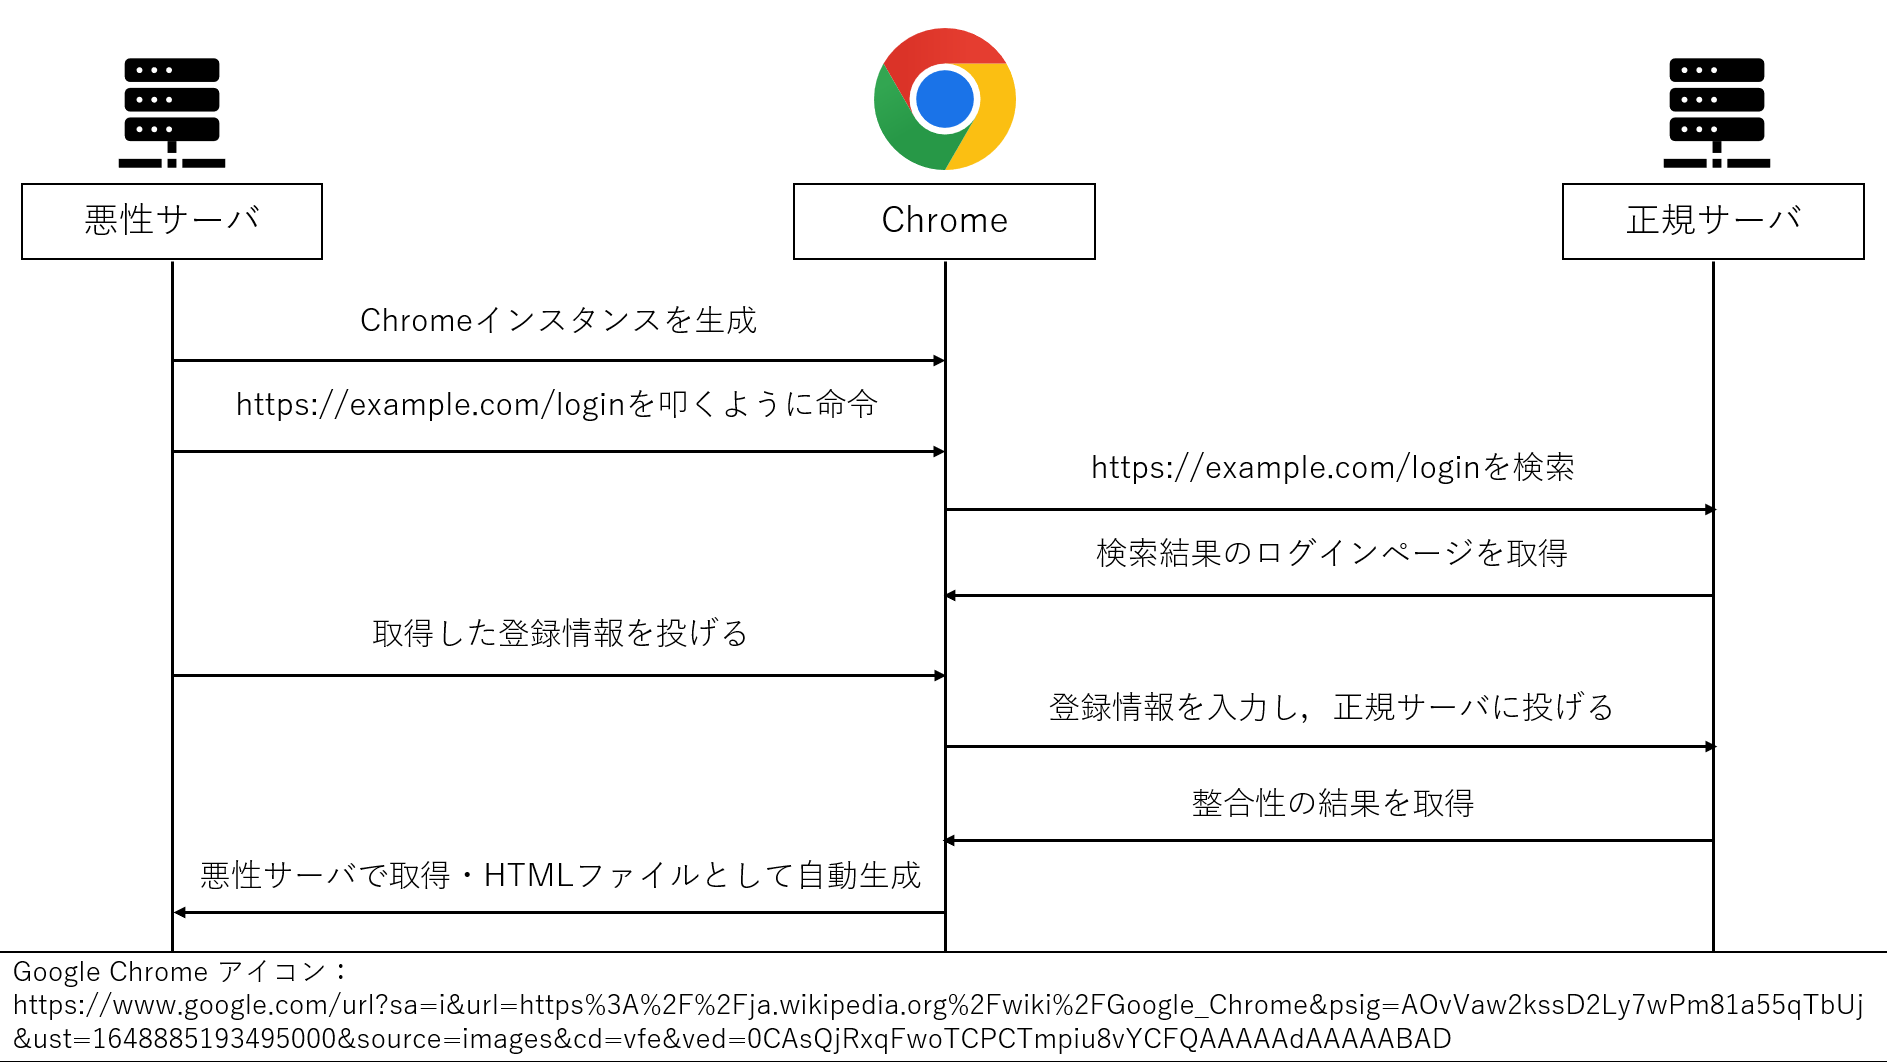
\includegraphics[width=15cm]{img/vc-vf-6-7.png}
                    \caption{登録情報の整合性の確認を行う流れ}
                    \label{flow-6-7}
                \end{figure}
                \clearpage
        \section{検証結果}
            検証結果は以下のようになった.
            \subsection{楽天の場合}
                \subsubsection{動作結果}
                \subsubsection{問題点}
            \subsection{Amazonの場合}
                \subsubsection{動作結果}
                \subsubsection{問題点}
        \section{考察}
            今回の結果から,
        \section{参考文献・サイト}
\end{document}